%# -*- coding: utf-8-unix -*-
%%==================================================
%% chapter02.tex for SJTU Master Thesis
%% based on CASthesis
%% modified by wei.jianwen@gmail.com
%% Encoding: UTF-8
%%==================================================

\chapter{建模与分析}
\label{chap:example}
线程放置策略决定了线程在NUMA节点之间的分布,进而影响锁在NUMA架构机器上的吞吐率。而对于层级锁来说,由于其本地偏好的锁传递规则的影响,线程放置策略还会影响其长期公平性。本章首先通过实验验证紧凑策略和平均策略在层级锁的吞吐率和长期公平性方面的表现,然后建模分析线程放置策略影响吞吐率和长期公平性的根本因素,进而得出线程放置策略优化应遵循的原则和面临的挑战。
\section{实验验证}
我们的实验跑在Intel Xeon E5上,该机器有四个NUMA节点组成,每个节点上包含八个计算核心。实验的benchmark取自libslock中的stress\_one,实验中用到的锁是cstmcs锁,该锁是一个两层的MCS锁,包括一个全局MCS锁和每个节点上的本地MCS锁。实验中stress\_one被配置为使用12个线程,每个线程重复以下操作:拿锁,写一定大小的缓存,放锁,暂停一段时间。该实验中我们用暂停时间的长短来控制锁的竞争强度的大小,暂停时间越长,锁的竞争越激烈,实验中用到了两个暂停时间:500时钟周期和5000始终周期。图\ref{Fig:compact}和图\ref{Fig:even}分别展示了该实验在紧凑和平均两种放置策略下单个线程的吞吐率,其中在平均放置策略中我们只是用了4个NUMA节点中的两个节点。上述两张实验图中每个长条代表单个线程的吞吐率,而不同颜色表示不同的竞争强度。表\ref{tab:aggregate}显示了不同配置下总的吞吐率。

\begin{table}[!hpb]
  \centering
  \bicaption[指向一个表格的表目录索引]
    {总吞吐率}
    {Aggregate Throughput}
  \label{tab:aggregate}
  \begin{tabular}{@{}llr@{}} \toprule
    吞吐率(acquisitions/s) & 紧凑放置 & 平均放置 \\ \midrule
    5000 cycles & 4574093 & 3101512 \\
    500  cycles & 4401877 & 4273903 \\
  \end{tabular}
\end{table}

从表\ref{tab:aggregate}中可以看出,两种竞争强度下的最高吞吐率比较接近,即增加单个线程的锁请求频率并未增加总的吞吐率,所以上述两种竞争轻度下cstmcs锁都已经达到了饱和。在锁达到饱和并且关键区域执行时间不变的情况下,影响总的吞吐率的最主要的因素将是锁传递的平均时延大小,而在NUMA架构下影响锁传递平均时延大小的主要是锁在NUMA节点之间传递的频率。

结合图\ref{Fig:compact}和表\ref{tab:aggregate}可以看出紧凑放置能够尽可能地保证层级锁地高吞吐率,但是总的吞吐率在线程之间地分布是严重不均衡地,同一个NUMA节点上地线程吞吐率基本相同,不同NUMA节点上地线程之间吞吐率差别可以达到十几倍,而且不同竞争强度下受益地线程集合正好相反。结合图\ref{Fig:even}和表\ref{tab:aggregate}可以看出平均放置尽可能地保证了层级锁地长期公平性,单个线程地吞吐率之间没有明显地差异,但是在竞争强度较小时其总的吞吐率相比紧凑放置有明显地损失,在不是严重吞吐率损失多大32.2\%。

\begin{figure}[t]
	\centering
	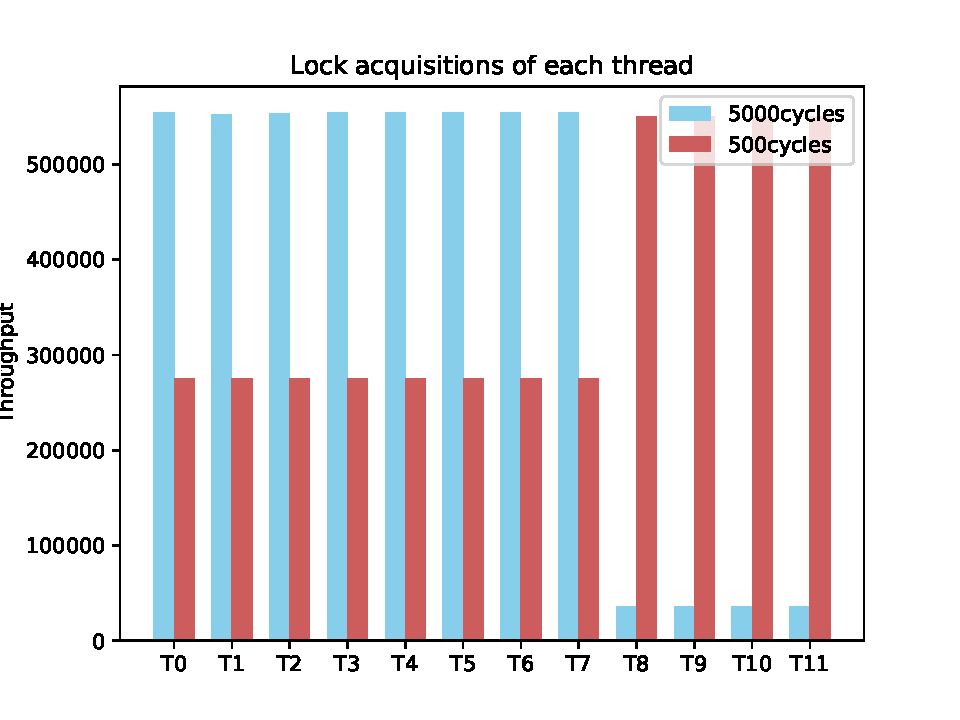
\includegraphics[width=5.6in]{compact.pdf}
	\caption{紧凑放置:单个线程的吞吐率}
	\label{Fig:compact}
\end{figure}

\begin{figure}[t]
	\centering
	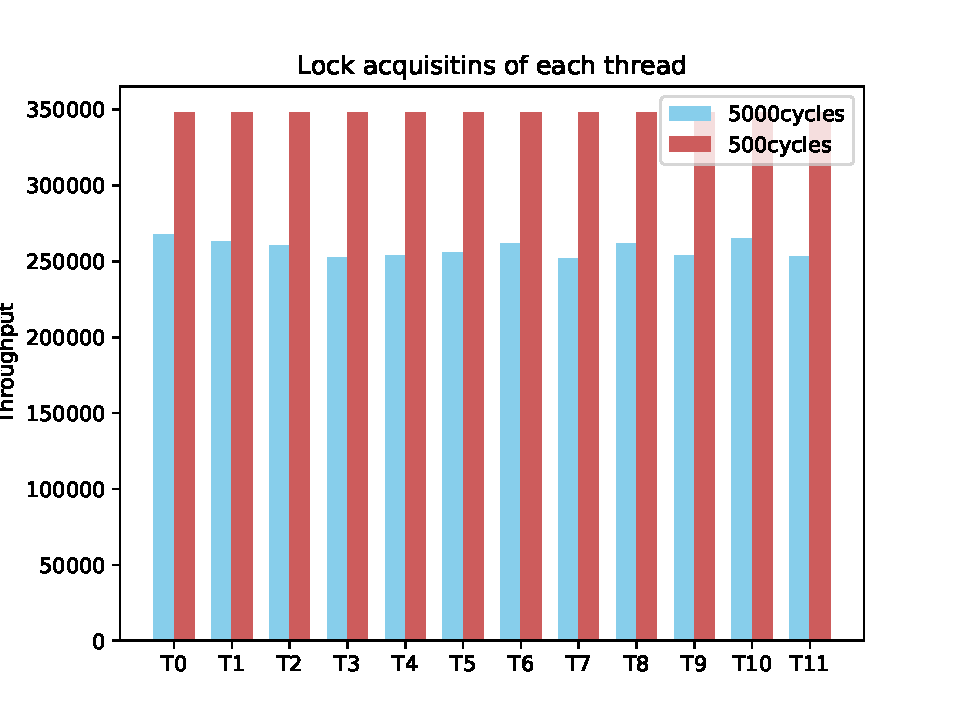
\includegraphics[width=5.6in]{even.pdf}
	\caption{平均放置:单个线程的吞吐率}
	\label{Fig:even}
\end{figure}

\section{单个线程的吞吐率}
以下我们按照层级锁地传递规则建模分析本实验用到的cstmcs锁中单个线程的吞吐率及影响其的主要因素。cstmcs锁中用到的全局锁和本地锁都是MCS锁,而MCS锁按照先进先出(FIFO,first in first out)的顺序在线程之间传递,所以我们可以认为全局MCS锁在相关NUMA节点之间按照round-robin的方式传递,当全局MCS锁传递到某个节点上时,对应的本地MCS锁也在该节点上运行的相关节点之间传递,如图\ref{Fig:circulation}所示。为了说明的方便,我们将全局MCS锁在所有相关节点之间传递一次的时间间隔定义为一个循环(circulation)。

\begin{figure}[t]
	\centering
	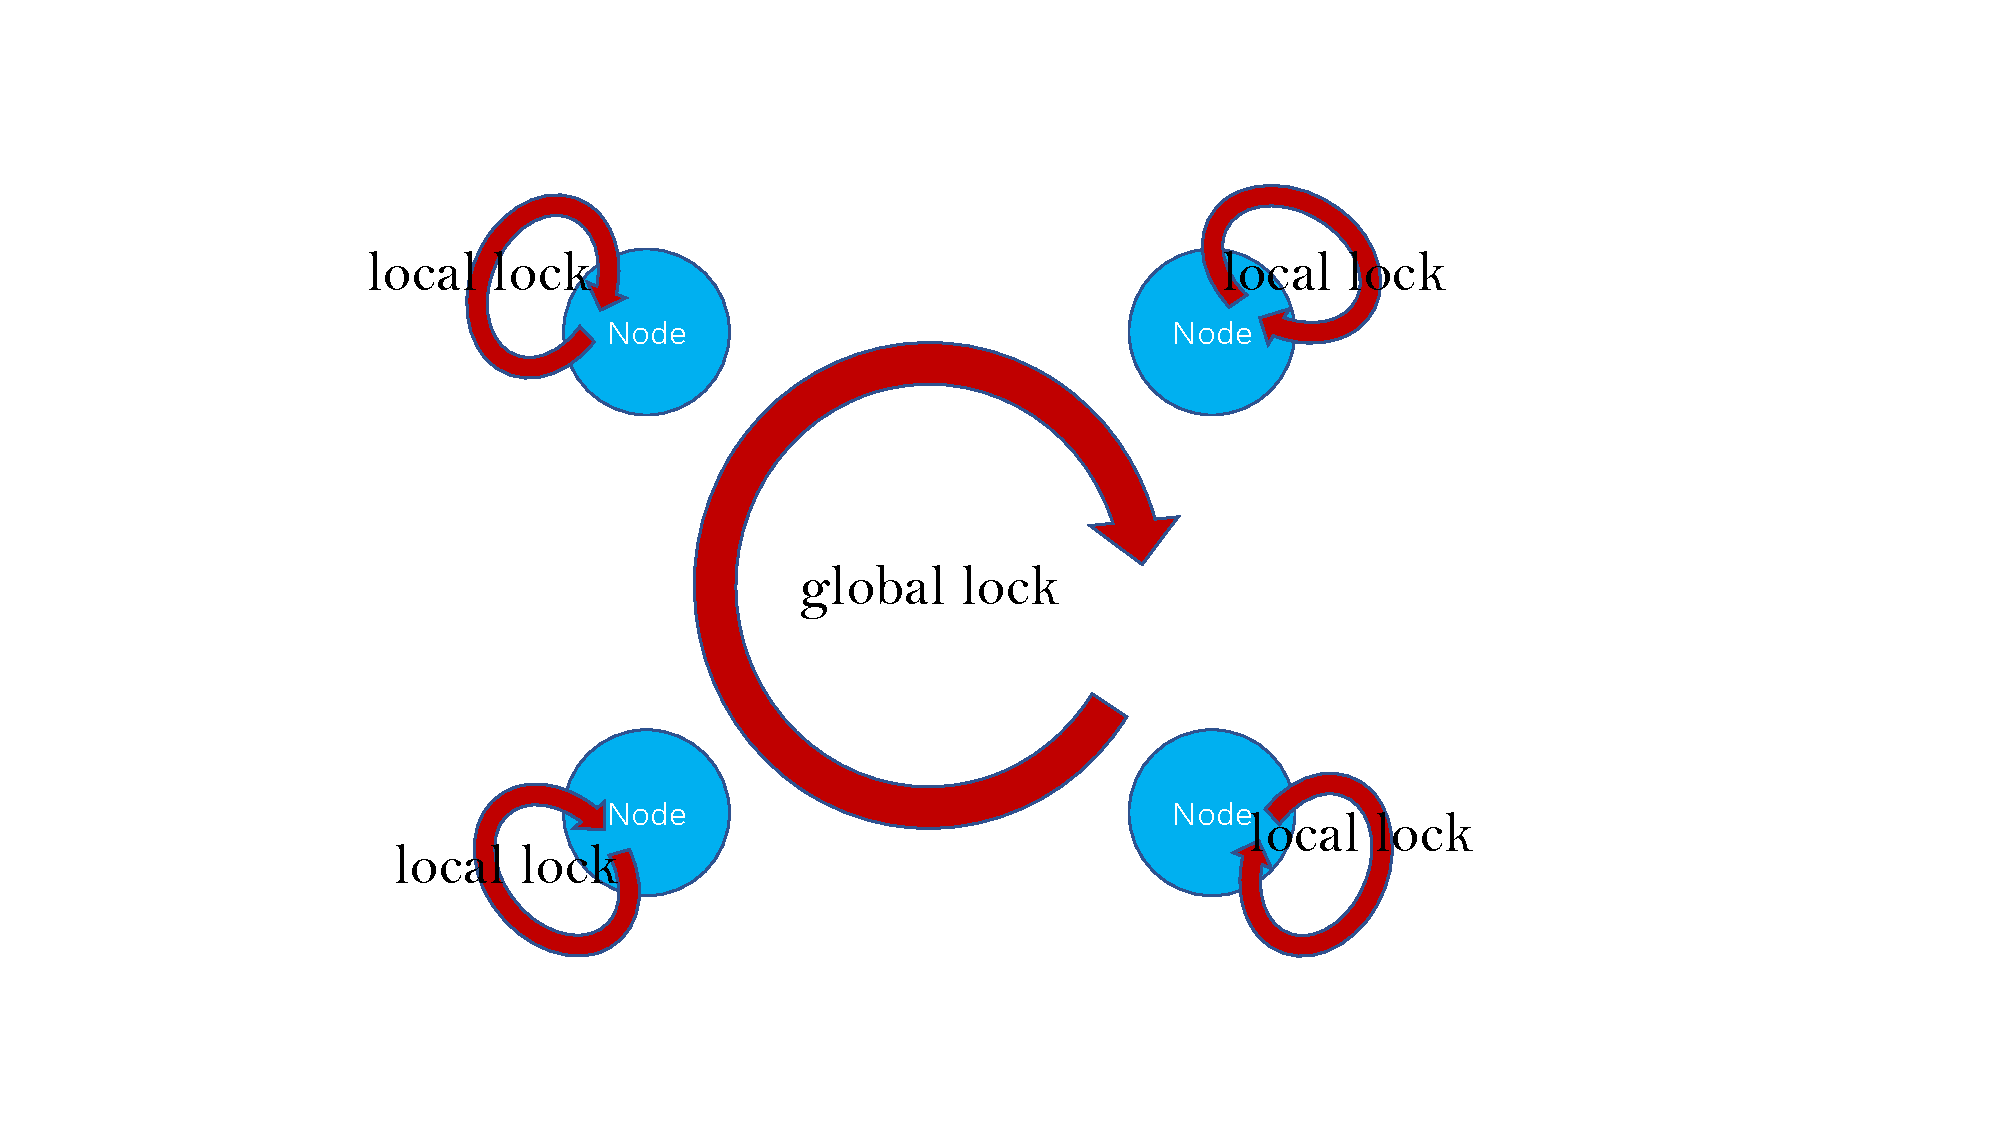
\includegraphics[width=5.6in]{circulation.pdf}
	\caption{cstmcs锁中的一个循环}
	\label{Fig:circulation}
\end{figure}

对于一个特定的线程来说,其在执行或者等待执行关键区域的概率可以表述为:
\begin{equation}\label{Eq:pro}
     P_{cs} = CS / (NCS + CS)
\end{equation}
其中CS和NCS分别代表关键区域和非关键区域的长度。

对于一个包含T个线程的应用来说,其在执行或者等待执行关键区域的线程数的期望值为:
\begin{equation}\label{Eq:expectation}
     E_{cs} = T * P_{cs}
\end{equation}

Ecs可以用来表示应用中的锁竞争强度,Ecs越大,锁的竞争轻度越大。我们按照Ecs的值大小将锁的状态定义为以下三种:
\begin{equation}\label{Eq:state}
Lock\ state =
\begin{cases}
under-saturated &\text{Ecs < 1}\\
saturated &\text{Ecs = 1}\\
over-saturated &\text{Ecs > 1}
\end{cases}
\end{equation}
其中饱和(saturated)是锁的一个特殊状态,如图\ref{Fig:saturation}所示,当锁处于饱和态时,锁被持续持有并且所有县城都能在请求锁的时候就拿到锁。否则或者锁不能被持续持有(欠饱和under-saturated)或者线程请求锁之后需要等待一段时间才能拿到锁(过饱和over-saturated)。

根据层级锁的传递规则,在每一个循环中,当某个NUMA节点上的线程使得该节点上的本地锁饱和或者过饱和时,层级锁就能够在该节点山一致传递直到总的传递次数达到预先设定的限制(threshold)为止;否则该节点上每个线程拿锁一次之后全局锁就会被其他节点拿走,该节点上锁的总传递次数将只有N,其中N是该节点上运行的线程数。即
\begin{equation}\label{Eq:localtrans}
local\ acqs =
\begin{cases}
N &\text{under-saturated}\\
threshold &\text{otherwise}
\end{cases}
\end{equation}
因为MCS锁是完全公平的,所以每个节点上运行的线程在一个循环里边的拿锁次数为
\begin{equation}\label{Eq:per}
acqs\_per\_thread =
\begin{cases}
1 &\text{under-saturated}\\
threshold / N &\text{otherwise}
\end{cases}
\end{equation}
\section{长期公平性}
我们定义两个线程之间的关系为对称(symmetric)如果不管锁的竞争强度如何变化,这两个线程理论上长期的拿锁次数差距为0. 那么由MCS锁的特性可知,运行在同一个NUMA节点上的任何两个线程之间是对称的;对于运行在两个不同节点上的线程来说,由公式\ref{Eq:per}可知只有当这两个节点上运行的线程数量相等时,这两个线程是对称的。另外,很明显对称关系是一种等价关系,因此所有竞争同一个层级锁的线程可以按照其在NUMA节点上的分布来被分为若干等价类。例如,图\ref{Fig:symmetric}中的20个线程可以分为两个等价类,其中节点0上的8个线程和节点3上的8个线程属于同一个等价类,剩下的4个线程属于另一个等价类。

显然只有所有线程都在同一个等价类时层级锁才对于所有线程来说都是长期公平的。这可以解释为什么图\ref{Fig:compact}中紧凑放置不能保证长期公平性,因为图\ref{Fig:compact}中的线程属于两个等价类。而两种竞争强度下受益线程集合互补则可以由公式\ref{Eq:per}来解释,当竞争强度较小(暂停时间为5000 cycles)时,前8个线程所在的节点的本地锁处于饱和或者国饱和态而后4个线程所在的节点的本地MCS锁处于欠饱和态,所以前8个线程的吞吐率远大于后四个线程的吞吐率;当竞争强度较大(暂停时间为500 cycles)时,两个节点上的本地MCS锁都处于饱和或者过饱和态,所以对于后四个线程更有利。

\begin{figure}[t]
	\centering
	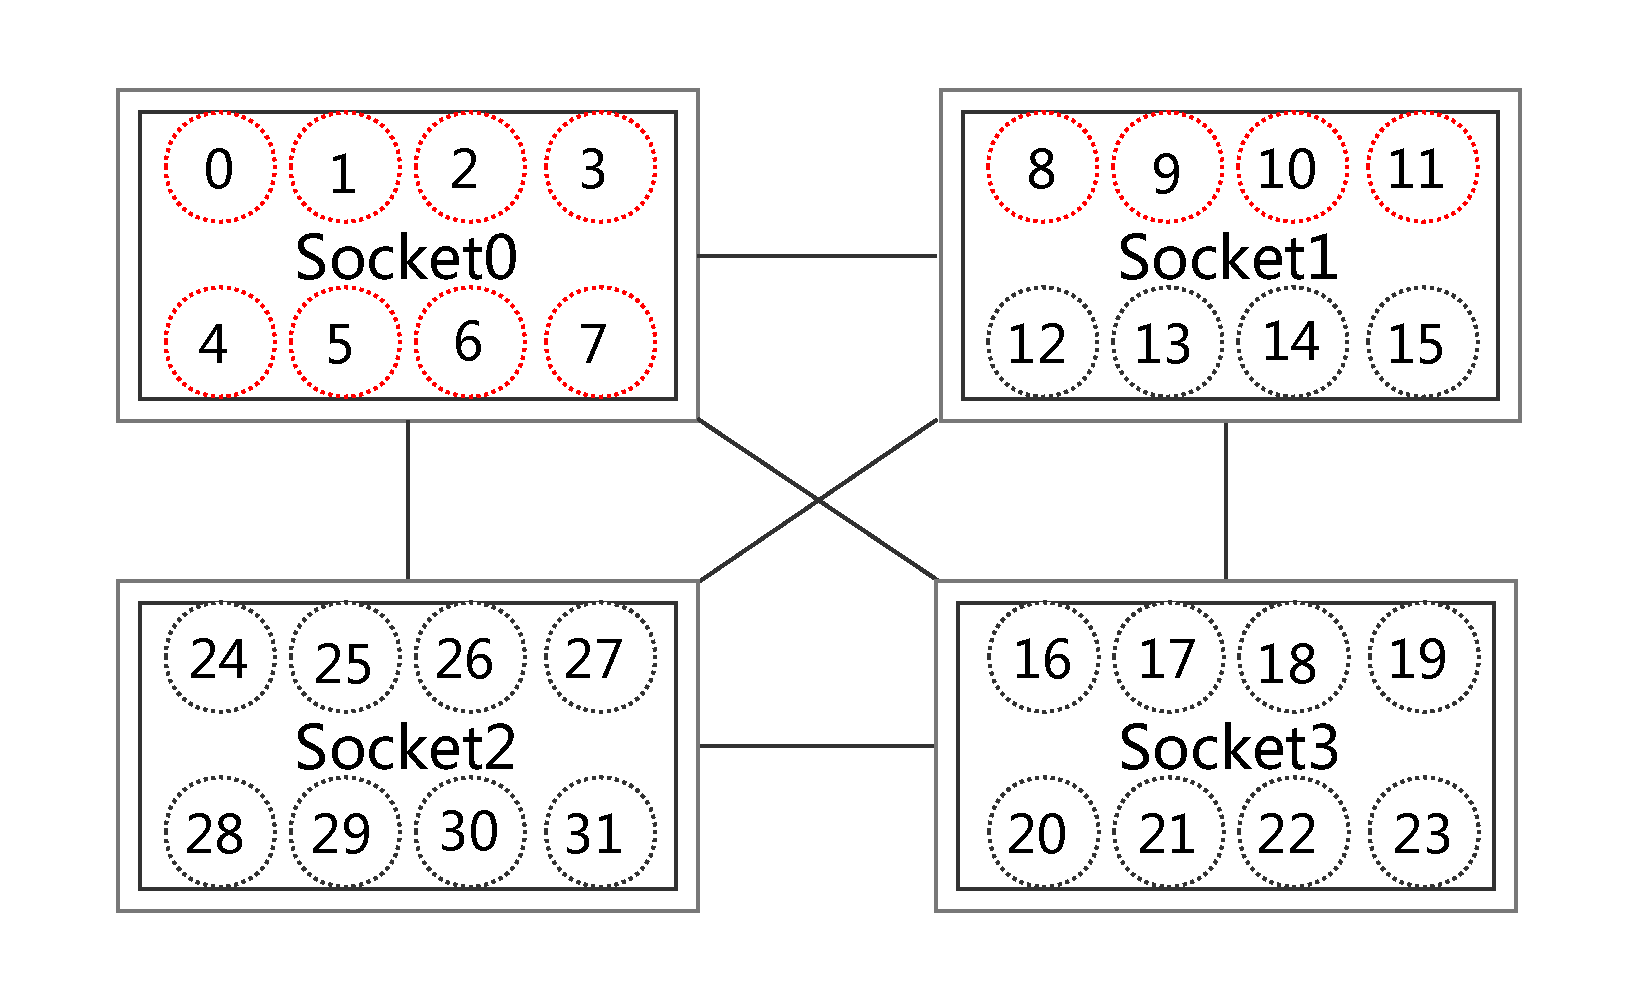
\includegraphics[width=5.6in]{symmetric.pdf}
	\caption{线程等价类}
	\label{Fig:symmetric}
\end{figure}

\section{总吞吐率}
在每个循环中,全局MCS锁在节点间的传递次数是固定的并且等于相关的节点数目,因此每个循环中单个线程的拿锁次数越多,锁在节点间传递的比例就越小,总吞吐率也就相应越高。根据公式\ref{Eq:per},在每个循环中,单个线程的吞吐率为1如果其锁在的节点的本地MCS锁是欠饱和的,否则其吞吐率为threshold/N, 一般情况下,threshold会是N的数倍,因此每个本地MCS锁是否达到饱和对于总的吞吐率有很大的影响。而根据公式\ref{Eq:pro}到公式\ref{Eq:state},保证局部MCS锁达到饱和的条件是在相应的节点上放置至少sat个线程,sat是Pcs的倒数
P\_{cs} as Equation\ref{Eq:sat} shows
\begin{equation}\label{Eq:sat}
     sat = (NCS + CS) / CS
\end{equation}
这儿sat正是饱和点的大小。这解释了为什么平均放置在竞争高(暂停时间500 cycles)时能获得与紧凑放置差不多的吞吐率而在竞争强度较低(暂停时间5000 cycles)是相比紧凑放置吞吐率严重下降。竞争强度高时对应饱和点小,而竞争轻度低时对应饱和点大,而上述实验中平均放置在每个节点上的线程数正好处于这两个饱和点之间。

\begin{figure}[t]
	\centering
	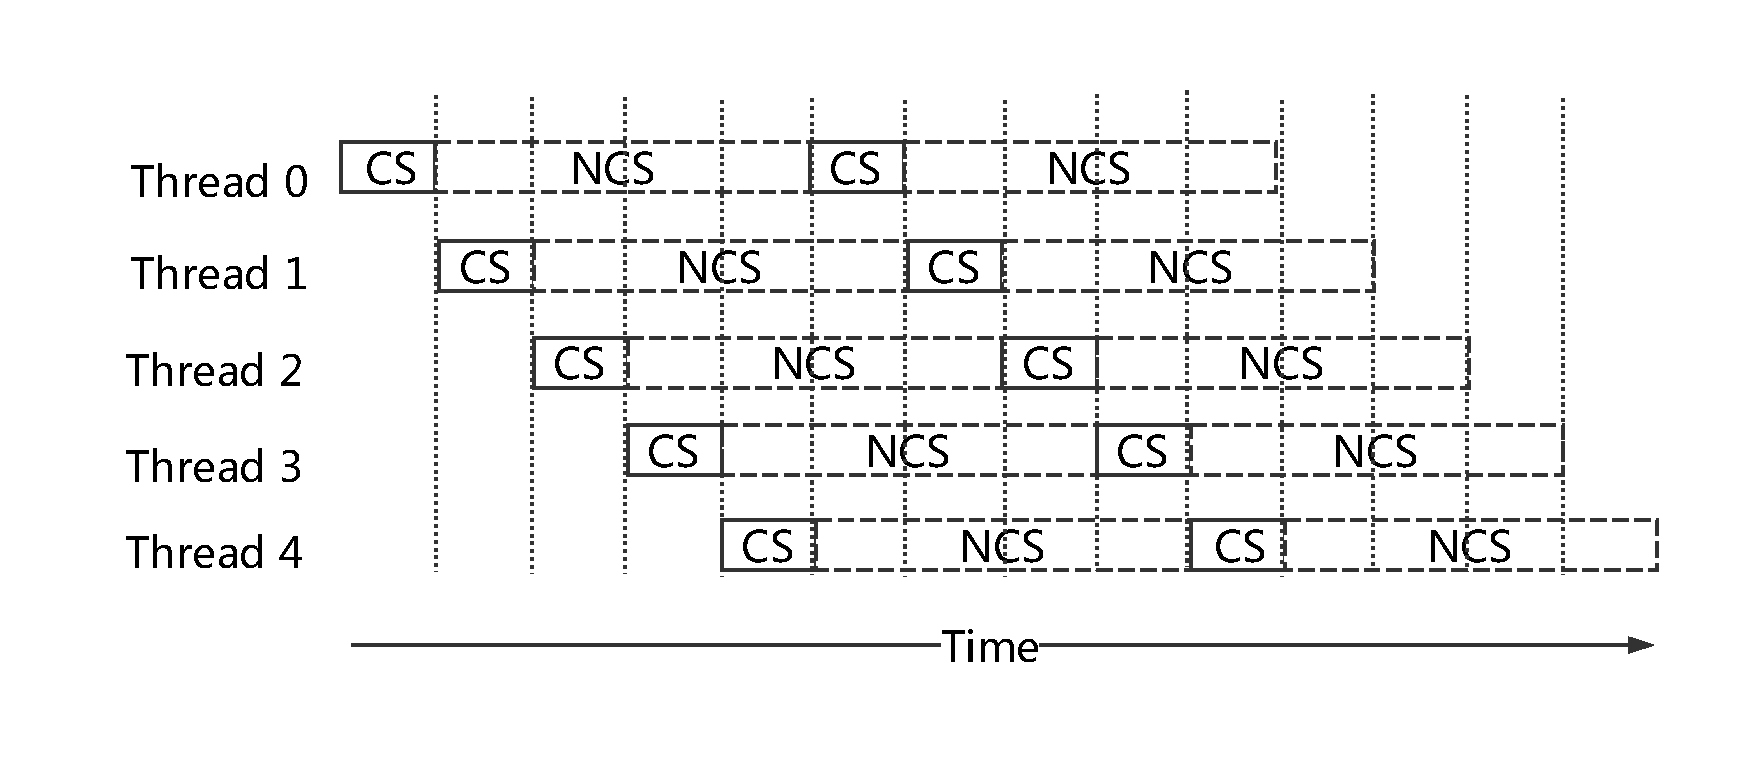
\includegraphics[width=5.6in]{saturation.pdf}
	\caption{饱和点,该图示中饱和点为5}
	\label{Fig:saturation}
\end{figure}

\section{结论与挑战}
通过上述建模和分析我们认为,从线程放置的角度来优化层级所的吞吐率和长期公平性应该遵循以下原则:
\begin{enumerate}
  \item 保证每个线程运行在一个专用核地前提下,使得线程分布在尽可能少地NUMA节点上;
  \item 尽可能保证放置在每个相关节点上地线程数达到或超过当前地饱和点;
  \item 尽可能使得每个相关节点上放置地线程数相等;
\end{enumerate}

上述原则中,第一点在避免抢占带来的相关问题地同时使得层级所能够更有效地挖掘核利用线程之间地亲和性来达到更高地吞吐率;第二点通过降低锁在节点间地传递比例来提高吞吐率,可以看作是第一点的延申;第3点通过使所有线程变为一个等价类来保证层级所的长期公平性。

紧凑放置遵循了前两点原则,保证了高吞吐率但是存在严重的长期不公平问题;平均放置遵循了第三点原则,保证了层级所的长期公平性但是存在吞吐率严重下降的问题。现实中很多应用场景比如公有云等对于吞吐率核公平性都有着很高的要求,现有的线程放置策略显然很难满足这些场景的需求。如果能同时满足上述三项原则,则可以同时保证层级所的吞吐率核长期公平性,然而现实中这三点很难同时满足甚至相互冲突,比如本章开始的实验在暂停时间为5000 cycles时,简单的放置并不能同时满足线程平均放置和每个节点上放置的线程数至少为饱和点的大小这两个条件;另外,现实中应用在运行过程中线程数和饱和点都可能会随着上层的需求或者下层硬件状态的变化而变化,简单的线程放置策略并不能总是保证吞吐率和长期公平性。上述两点是本文锁面临的主要挑战,显然,简单的线程放置策略很难解决上述挑战,我们需要额外的技术和更细力度的线程放置来应对这些挑战。